\section{PURR}
\label{sPURR}
\index{PURR|textbf}
\index{unresolved resonance range}

\hypertarget{sPURRhy}{The}
unresolved self-shielding\index{self-shielding} data generated
by \hyperlink{sUNRESRhy}{UNRESR}\index{UNRESR} are
suitable for use in multigroup methods
after processing by \hyperlink{sGROUPRhy}{GROUPR}\index{GROUPR},
but the so-called
Bondarenko method\cite{Bondarenko}\index{Bondarenko method}
is not very useful for continuous-energy Monte Carlo\index{Monte Carlo}
codes like MCNP\cite{MCNP}.\index{MCNP}  As pointed out by
Levitt\cite{levitt},\index{Levitt} the natural approach for treating
unresolved-resonance self-shielding for
Monte Carlo codes is the ``Probability Table'' method.
\index{probability tables}  The method requires tables of
the probability that the total cross section will be less than some
value $\sigma_t$ for a number of incident energies.  Then, when the
Monte Carlo code needs the cross section at $E$, it selects a
random number between 0 and 1 and looks up the corresponding $\sigma_t$
in the appropriate probability table.  The corresponding capture and
fission cross sections are obtained from conditional probability
tables that give $\sigma_\gamma$ and $\sigma_f$ versus $\sigma_t$.
This approach allows geometry and mix effects on self-shielding to
arise naturally during the Monte Carlo calculation, and it supplies
reasonable variances for the tallies.  The probability table method
has been used successfully in a number of applications, notably the VIM
continuous-energy Monte Carlo code\cite{vim},\index{VIM} which was
developed to solve fast-reactor problems where unresolved effects
become very important.

The PURR module produces probability tables that can be used in
versions of MCNP from 4B on to treat unresolved-resonance
self-shielding.

In recent versions of NJOY, the Bondarenko self-shielded cross sections
from PURR will override any previous self-shielded data on the
PENDF file coming from \hyperlink{sUNRESRhy}{UNRESR}.

This chapter describes the PURR module in NJOY2016.0.

\subsection{Sampling from Ladders}
\label{ssPURR_ladder}

In the unresolved range, we don't know the real center energy of any of
the resonances, and we don't know the partial widths that determine the
shape and strength of any particular resonance.  However, the ENDF
evaluation provides us with mean values for the resonance spacings,
the probability distribution for the spacings (the Wigner distribution),
\index{Wigner distributions} the mean values for the resonance partial
widths, and the distributions for the partial widths (chi-square
distributions\index{chi-square distributions} for various numbers
of degrees of freedom).  These quantities are given for several
different spin sequences, which are statistically independent, and
for a number of energies spaced through the unresolved energy range.
A ``narrow-resonance assumption'' is always made in the unresolved
range; that is, the energy loss in scattering in the system is
assumed to be large with respect to the width of any of the resonances.
Thus, neutrons arrive at random energies that are not correlated
with the resonance structure.  The effective cross sections at one of
the energies in the ENDF unresolved grid then depend on a number of
resonances in the vicinity of that energy, all of which are assumed to
have resonance parameters characteristic of that grid energy value.

This allows us to define a plausible set of cross sections in the
vicinity of one of the grid energies.  We first define an energy range
that will hold a specified number of resonances, and we randomly
choose a set of sampling energies in this range, avoiding the
ends of the range to reduce truncation effects.  For each spin
sequence, we start by choosing a center for the starting resonance from
a uniform distribution (this provides a random offset between the
various spin sequences in the ladder).  We then choose a set of partial
widths for this resonance drawn from the appropriate distributions.
A second resonance is then chosen above the first using the distribution
for resonance spacings, and partial widths are randomly chosen for it.
Then a third resonance is chosen, and so on, until the energy range
defined for the ladder has been filled.  We can now compute the
cross section contributions from this spin sequence at each of the
sampling energies.  We then step to the next spin sequence and repeat
the process.  After looping through all the spin sequences, the
accumulated cross sections are one possible set of plausible cross
sections that obey the defined statistics for the unresolved range.

We can now go through this set of sampled cross sections,
determine how many values of the total cross section hit each bin,
and compute the conditional average for the elastic, fission, and
capture cross sections for samples where the total ends up in each
bin.  This is the contribution to the probability table from the
particular resonance ladder.  However, using only one ladder could
result in average cross sections that differ dramatically from the
expected infinitely dilute averages computed directly from the
resonance parameters.  Therefore, the whole sampling process is
repeated again for a user-selected number of different ladders.
When enough ladders have been processed, the average cross sections
will begin to converge to the expected results.  The following
piece of a PURR output listing shows 16 ladders being processed for
$^{235}$U from ENDF/B-VII.0:

\newpage
\small
\begin{ccode}

e= 2.2500E+03   spot= 1.1700E+01   dbar= 1.6137E-01   sigx= 0.0000E+00
             total     elastic     fission     capture
     1  1.9471E+01  1.2074E+01  5.3460E+00  2.0507E+00
     2  1.9617E+01  1.2041E+01  5.6196E+00  1.9566E+00
     3  1.9559E+01  1.2075E+01  5.4597E+00  2.0245E+00
     4  1.9458E+01  1.2000E+01  5.5723E+00  1.8859E+00
   ...
    14  1.9456E+01  1.2102E+01  5.3632E+00  1.9905E+00
    15  1.9660E+01  1.2082E+01  5.4429E+00  2.1354E+00
    16  1.9363E+01  1.2019E+01  5.3736E+00  1.9710E+00
  bkgd  0.0000E+00  0.0000E+00  0.0000E+00  0.0000E+00
  infd  1.9778E+01  1.2105E+01  5.6364E+00  2.0363E+00
  aver  1.9567E+01  1.2068E+01  5.5030E+00  1.9964E+00
  pcsd        1.38        0.32        3.28        4.97
  nres        3664

\end{ccode}
\normalsize

\noindent
Some steps have been eliminated for brevity.  The ``aver'' values
computed from the sampling have converged to be fairly close to the
infinitely dilute values ``infd'' computed from the resonance
parameters.  Here \cword{spot} is the potential scattering cross
section, \cword{dbar} is the average resonance spacing, and
\cword{sigx} is the competitive cross section.

The probability table can be used to generate a picture of the
probability distribution for the total cross section as shown
in Fig.~\ref{totpd}.  This example is for $^{238}$U.  It demonstrates
how the fluctuations get smaller as energy increases, which means
that the self-shielding effect also gets smaller.
\index{probability distribution for total}

\begin{figure}[thb]\centering
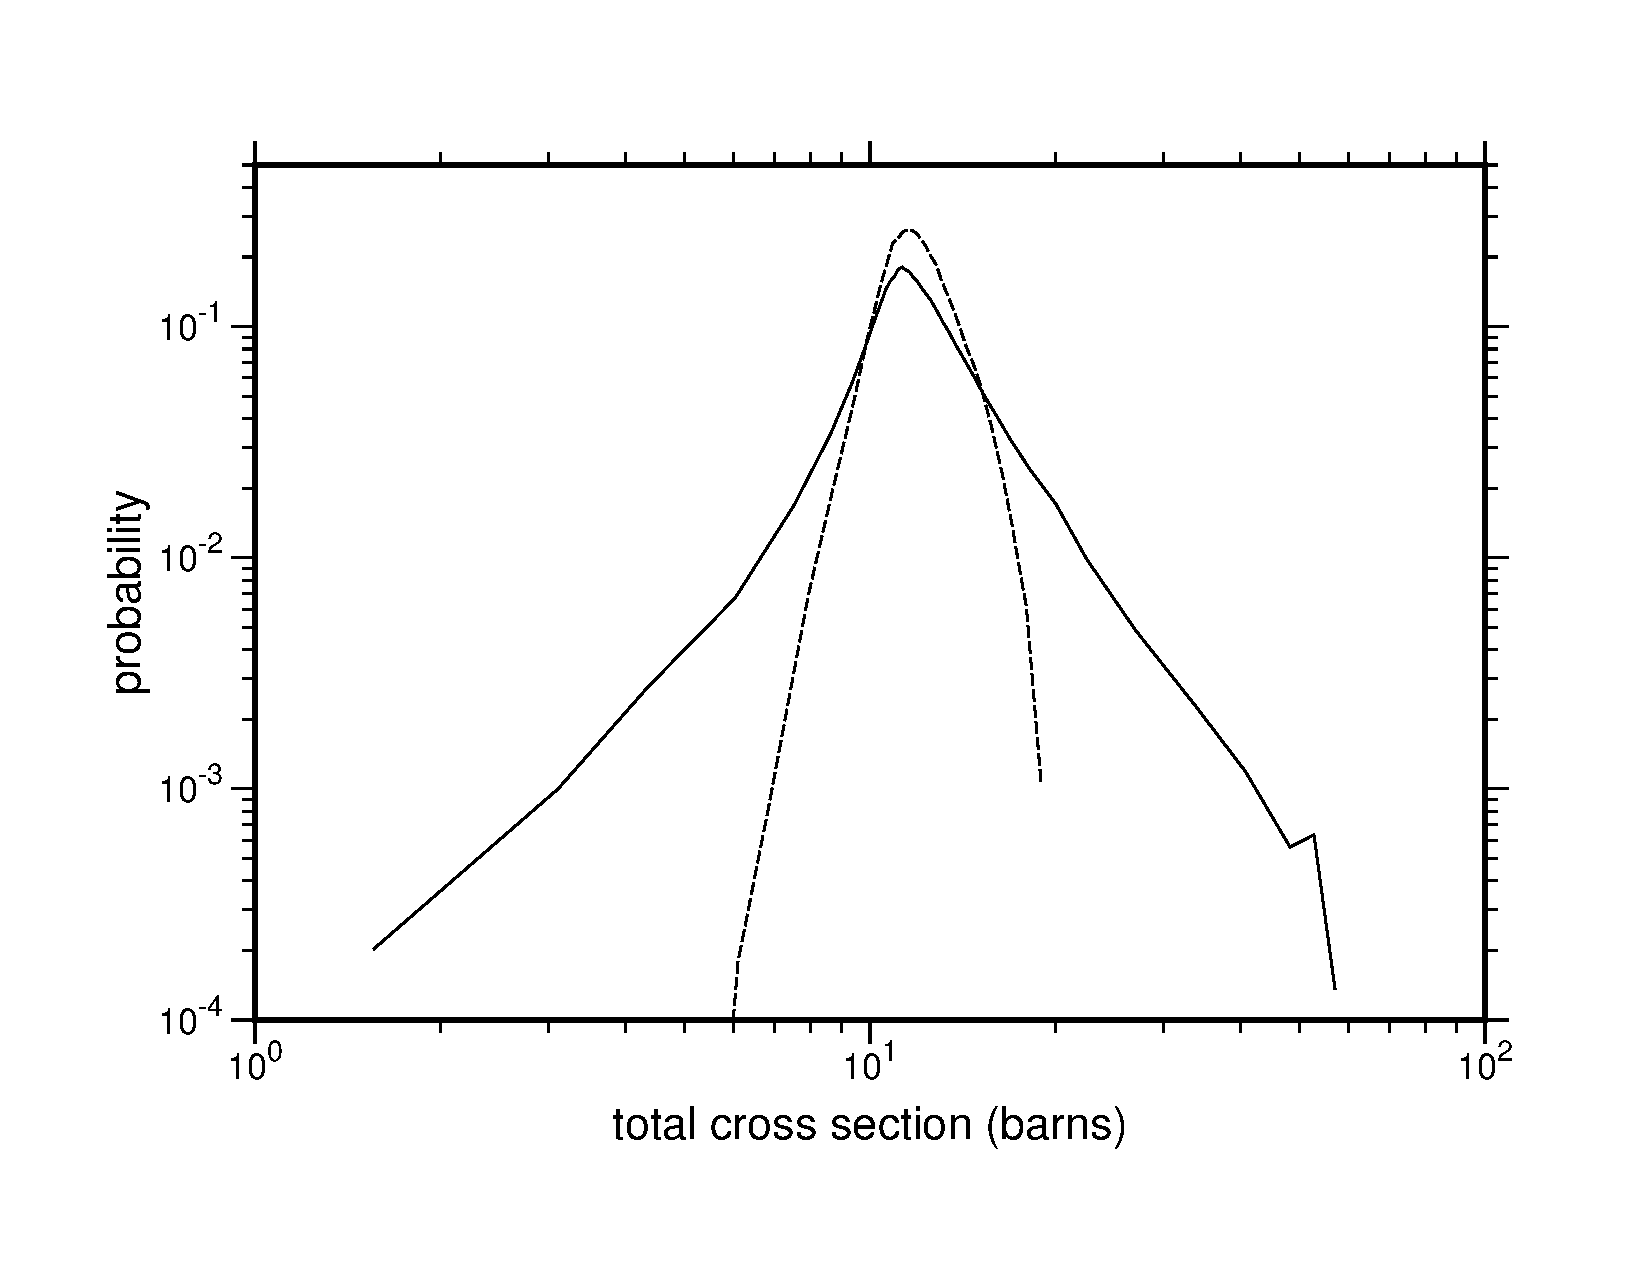
\includegraphics[keepaspectratio, height=3.8in, angle=0]{figs/totpdack}
\caption[Sample total cross section probability distributions]{The
 probability distribution for the total cross section at 20 keV (solid) and
 140 keV (dashed) in the unresolved resonance range of $^{238}$U.}
\label{totpd}
\end{figure}

The statements that generate the \hyperlink{sVIEWRhy}{VIEWR}
input for this kind of
plot are normally commented out.

During the sampling process, PURR also computes Bondarenko-style
self-shielded cross sections just like those produced by
\hyperlink{sUNRESRhy}{UNRESR}\index{UNRESR}.  These
values are printed out so that they
can be compared with the results from other methods.  For recent
versions of NJOY, the Bondarenko self-shielded cross sections
replace any previous values on the PENDF file from
\hyperlink{sUNRESRhy}{UNRESR}\index{UNRESR}.
The Bondarenko cross sections can also be computed directly from
the probability table using

\begin{equation}
   \sigma_x(E)=\frac{\displaystyle\sum_i \frac{P_i(E)\sigma_{xi}(E)}
     {\sigma_0+\sigma_{ti}(E)}}
      {\displaystyle\sum_i \frac{P_i(E)}{\sigma_0+\sigma_{ti}}} \,,
\end{equation}

\noindent
where $x$ can be $t$ for total, $n$ for elastic, $f$ for fission, or
$\gamma$ for capture.  These values are also printed out.  They can
be compared to the Bondarenko values from direct sampling to help
judge whether adequate convergence has been obtained.

Fig.~\ref{u238ss} shows Bondarenko-style self-shielded curves
from PURR for the total cross section for $^{238}$U in the unresolved
region at three different values of the dilution.  This kind of plot
is included in the standard graphs generated by
\hyperlink{sACERhy}{ACER}.  Most
of the self shielding comes from the elastic channel in this case.
Fig.~\ref{u238sf} shows how the total self-shielding factor for
$^{238}$U varies with temperature and dilution at an energy of 20 keV.

\begin{figure}[t]\centering
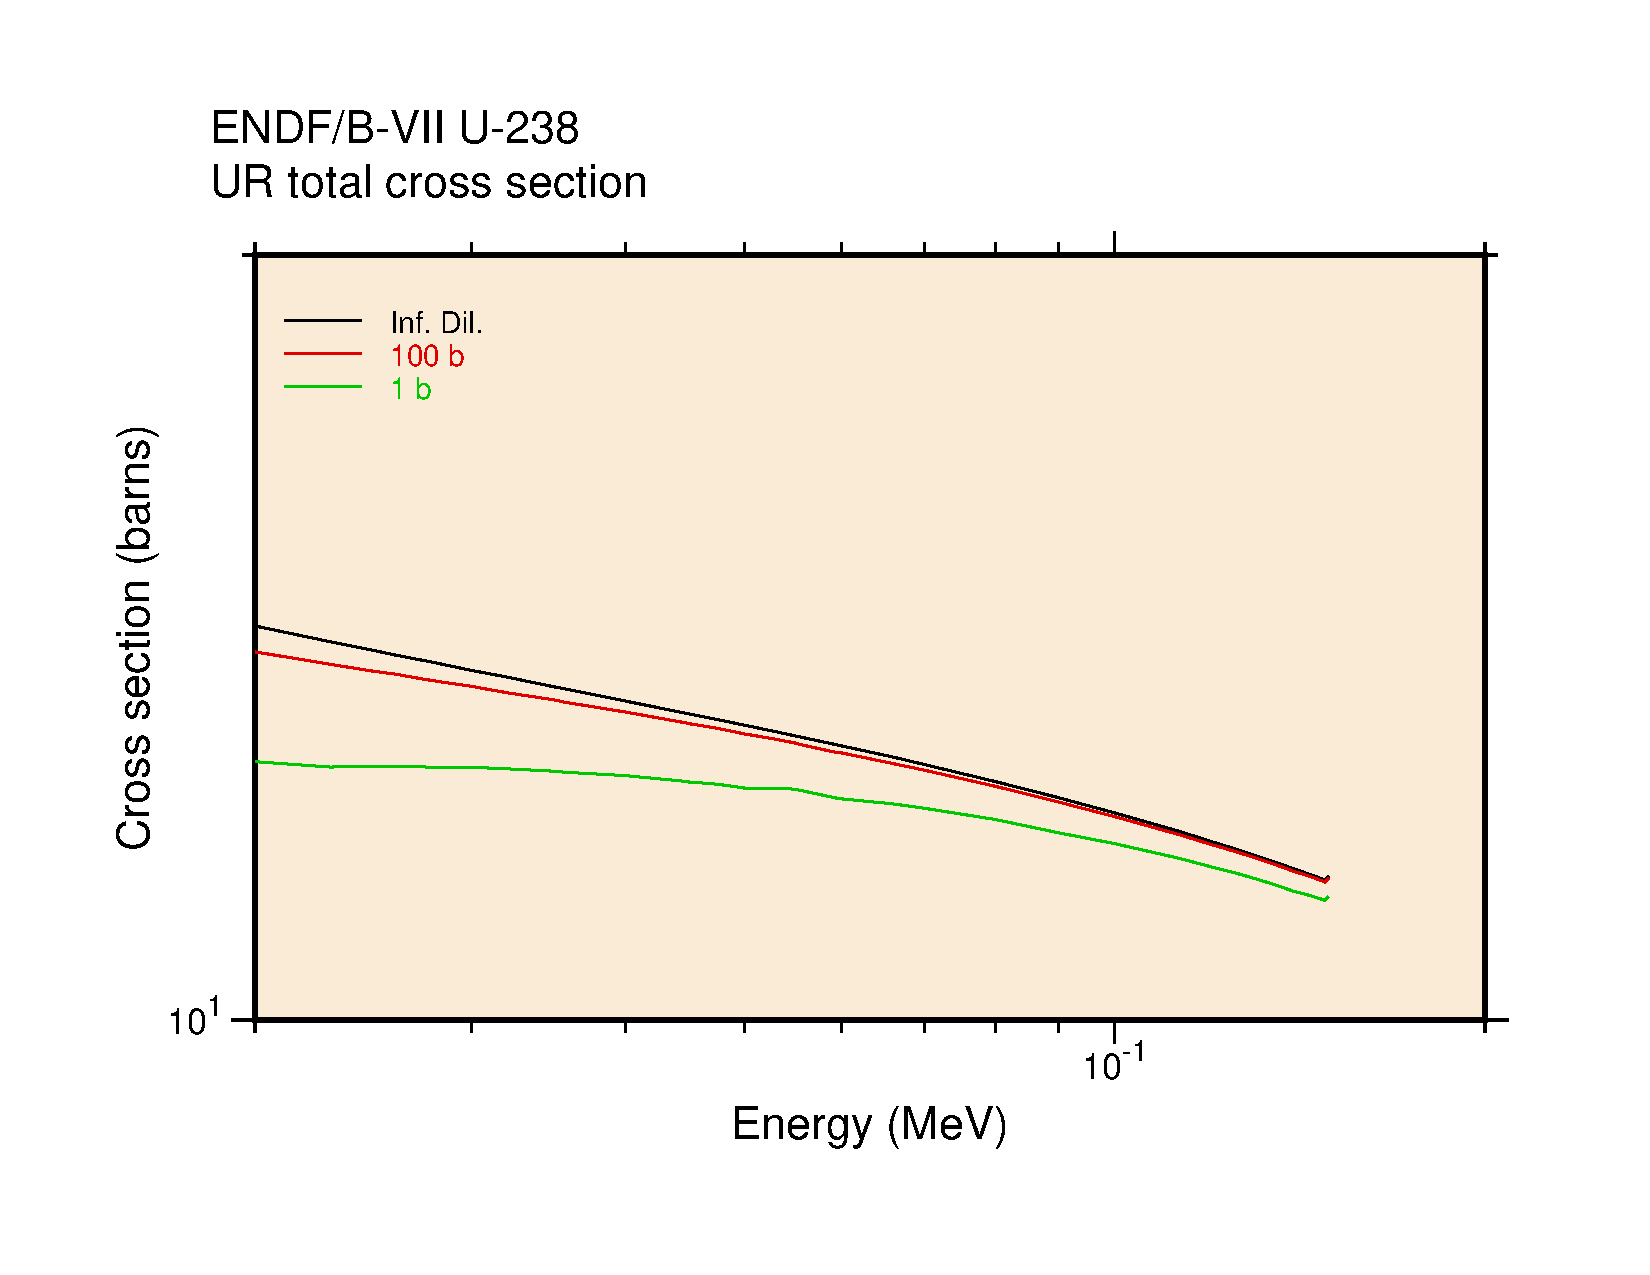
\includegraphics[keepaspectratio, height=3.8in, angle=0]{figs/u238ssack}
\caption[Bondarenko-style self-shielding]{Bondarenko-style self-shielded
 cross sections for the total cross section of $^{238}$U in the unresolved
 resonance region at three different dilutions.}
\label{u238ss}
\end{figure}

\begin{figure}[t]\centering
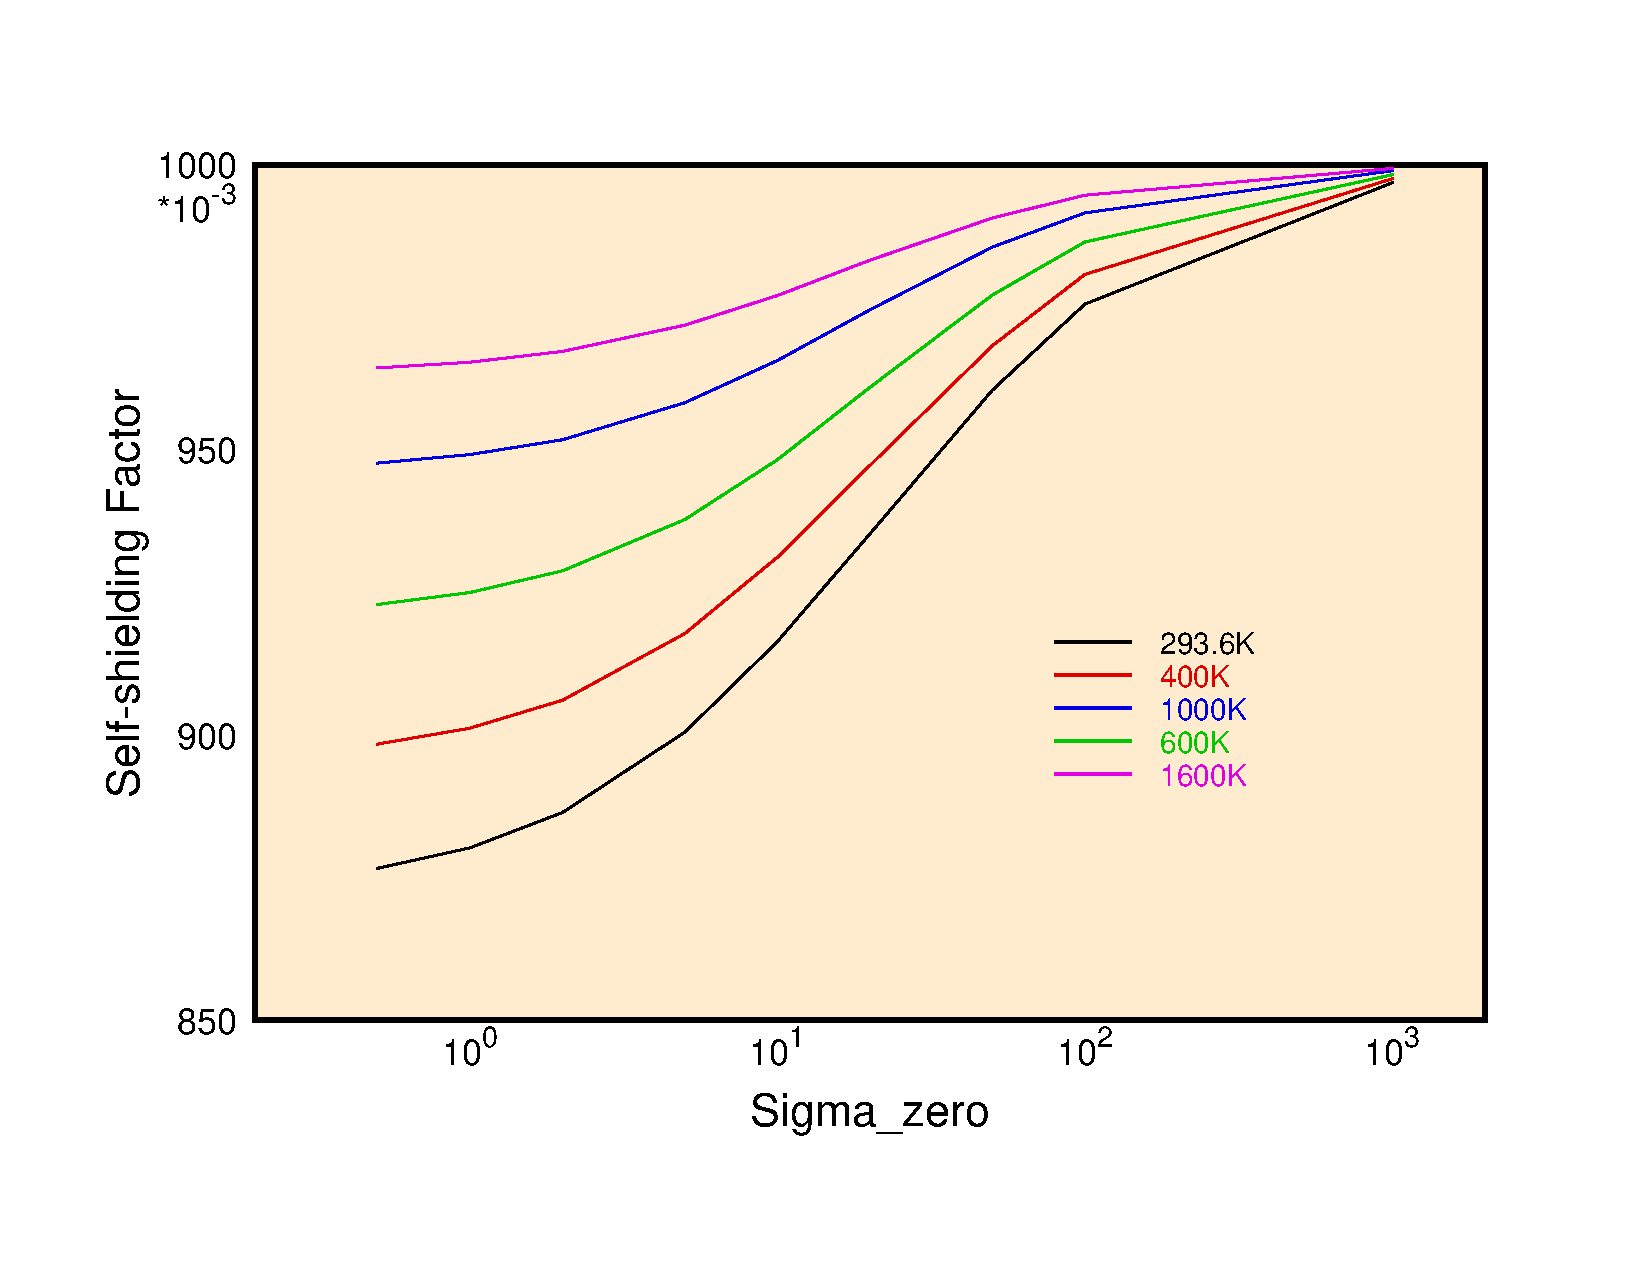
\includegraphics[keepaspectratio, height=3.8in, angle=0]{figs/u238sfack}
\caption[Self-shielding variation with temperature and dilution]{Self-shielding
 factors for the total cross section of $^{238}$U at 20 keV
 showing the variation with temperature and background
 cross section (dilution).}
\label{u238sf}
\end{figure}

PURR uses the Single-Level Breit-Wigner\index{Single-Level Breit-Wigner}
(SLBW)\index{Single-Level Breit-Wigner!SLBW} approximation to calculate
cross sections (as specified for ENDF unresolved data), and it uses
the $\psi{-}\chi$ method\index{$\psi\chi$ broadening}
to compute the Doppler broadened values.
As is well known, this method doesn't always produce reasonable
results for the small cross sections between resonances due to the
neglect of interference and multi-channel effects.  It is even
possible to get negative elastic cross sections.  When comparing
Bondarenko results from PURR with those from
\hyperlink{sUNRESRhy}{UNRESR}\index{UNRESR},
several factors should be considered.  The PURR results may be
more reliable at low $\sigma_0$ values than
\hyperlink{sUNRESRhy}{UNRESR} results because
of the more complete treatment of resonance overlap effects, but
the unrealistic cross sections in the dips between resonances will
eventually make even the PURR results suspect at low values.  This
effect may be especially apparent for the current-weighted
total cross section, which is especially sensitive to the
low cross sections between resonances.

The following piece of a PURR output listing shows the probability table
for the $^{235}$U example at an energy of 2.25 keV:

\newpage
\small
\begin{ccode}
 probability table
 tmin           1.162E+01
 tmax           1.352E+01  1.428E+01  1.509E+01  1.594E+01  1.683E+01 ...
                2.339E+01  2.471E+01  2.611E+01  2.758E+01  2.913E+01 ...
 prob           2.084E-02  3.597E-02  5.978E-02  8.244E-02  9.788E-02 ...
                6.094E-02  5.269E-02  4.169E-02  3.112E-02  1.806E-02 ...
 tot 2.936E+02  1.308E+01  1.393E+01  1.469E+01  1.552E+01  1.639E+01 ...
                2.275E+01  2.403E+01  2.537E+01  2.680E+01  2.832E+01 ...
 els 2.936E+02  1.114E+01  1.132E+01  1.144E+01  1.151E+01  1.161E+01 ...
                1.220E+01  1.230E+01  1.262E+01  1.274E+01  1.287E+01 ...
 fis 2.936E+02  1.486E+00  1.976E+00  2.444E+00  3.002E+00  3.582E+00 ...
                7.838E+00  8.607E+00  9.206E+00  1.023E+01  1.104E+01 ...
 cap 2.936E+02  4.574E-01  6.334E-01  8.095E-01  1.005E+00  1.202E+00 ...
                2.711E+00  3.121E+00  3.543E+00  3.832E+00  4.417E+00 ...

\end{ccode}
\normalsize

\noindent
The columns give the results for the 20 probability bins, but the
rightmost 5 columns of numbers have been removed to make the lines fit
this page.  Thus, we are seeing bins 1-5 and 11-15. The rows for
\cword{tmax} give the upper bounds for the total cross section bins,
and \cword{prob} gives the probability that the total cross section
lies in the bin.  The \cword{tot}, \cword{els}, \cword{fis}, and
\cword{cap} lines give the average cross section seen when the
total lies in that bin, all for a temperature of 293.6K.

The ENDF format contains an option called LSSF.  When LSSF=1, the
resonance parameters are to be used to compute a fluctuation factor
or self-shielding factor that is to be applied to the cross section
given in File 3 of the ENDF tape.  When LSSF=0, the parameters are
used to compute cross sections that are to be added to any possible
background corrections that may be given in File 3.  The presence of
this option doesn't effect the table printed out by PURR, but when
LSSF=1, all the cross section values are divided by the corresponding
infinitely dilute cross sections before the output file is written.
The bins then contain dimensionless fluctuation factors instead of
cross sections in barns.

\subsection{Temperature Correlations}
\label{ssPURR_temp}

One important feature of PURR is its ability to handle temperature
correlations\index{temperature correlations}.  If the Monte Carlo
code is tracking a particle through a system, it periodically checks
for a total cross section to calculate the range to the next
collision.  Consider a collision that takes place in a region
at a particular temperature.   The Monte Carlo code samples
from the probability table, getting a low cross section.  The
mean free path then takes the particle into another region
at a different temperature that contains the same material.
The sampled total cross section there cannot be independent from the
first; the resulting cross section must also be low.  PURR handles
this kind of correlation.  When a particular ladder of resonances
is sampled to obtain a probability table, all the different
temperatures are sampled simultaneously at the same energies to
preserve the correlations.  In the Monte Carlo code, it is only
necessary to use the same random number to sample for the cross section
in the two different regions to preserve the proper correlations.


\subsection{Self-Shielded Heating Values}
\label{ssPURR_self}

PURR can also provide self-shielding effects for the heating if
partial heating cross sections are provided to it from
\hyperlink{sHEATRhy}{HEATR}\index{HEATR}.  Of course,
there are no resonance parameters
for heating, but the heating value does depend on the elastic,
fission, and capture cross sections in the unresolved range.  It
may also have a contribution from competitive reactions, such as
MT=51 discrete inelastic scattering or (n,p) absorption.  The general
idea is to extract the portion of the heating corresponding to
elastic, fission, and heating, and to apply the fluctuations in
the probability table to them in order to get an estimate for
the possible fluctuations in the total heating.  This requires
that \hyperlink{sHEATRhy}{HEATR} be run to generate
the partial heating values MT=302
(elastic), MT=318 (fission), and MT=402 (capture), in addition
to the normal MT=301 (total heating).  With these present, each
partial heating value (eV-barns) can be divided by the
corresponding infinitely-dilute reaction cross section to
get eV/reaction for that reaction channel.  These numbers can
then be multiplied by the corresponding conditional cross section
in each bin of the probability table and added to the eV-barns from
the competitive reaction, if any, to get a value for heating in
eV-barns in each bin.  Finally, these values can be divided by the
average total for the bin to get a heating value in eV/reaction that
MCNP can use with sampled values of the total cross section to
produce contributions to heating tallies.


\subsection{Random Numbers}
\label{ssPURR_random}

The version of PURR in NJOY2012 and continuing in NJOY2016 uses the
Fortran-based random number generator \cword{rann}.  Earlier versions
relied on random number generators from the host systems, but this
resulted in different answers from every machine and made it hard to do
Quality Assurance (QA) on PURR results.  The new approach allows
comparisons to be made with standard ``diff" utilities.  Different
machines should give the same results unless real changes are made.

\subsection{User Input}
\label{ssPURR_inp}

The following user input specification was copied from the comment
cards at the beginning of the PURR source.  It is always a good idea to
check these comments in the current version in case there have
been changes.
\index{PURR!PURR input}

\small
\begin{ccode}

   ! card 1
   !   nendf   unit for endf tape
   !   nin     unit for input pendf tape
   !   nout    unit for output pendf tape
   ! card 2
   !   matd    material to be processed
   !           matd=0 terminates purr
   !   ntemp   no. of temperatures (default=1)
   !   nsigz   no of sigma zeros (default=1)
   !   nbin    no. of probability bins
   !   nladr   no. of resonance ladders
   !   iprint  print option (0=min, 1=max, def=1)
   !   nunx    no. of energy points desired (def=0=all)
   ! card 3
   !   temp    temperatures in Kelvin (including zero)
   ! card 4
   !   sigz    sigma zero values (including infinity)

\end{ccode}
\normalsize

\noindent
The following is an example of \hyperlink{sHEATRhy}{HEATR}
and PURR input for a full
calculation of the probability tables for a fissionable material.
This would be just a small part of a sequence for producing a
PENDF file for $^{235}$U.

\small
\begin{ccode}
    ...
    heatr
    -21 -24 -25/
    9228 5/
    302 318 402 443 444/
    purr
    -21 -25 -26
    9228 8 7 20 32/
    293.6 400 600 800 1000 1200 1600 2000/
    1e10 1e4 1e3 300 100 30 10/
    0/
    ...

\end{ccode}
\normalsize

\noindent
The \hyperlink{sHEATRhy}{HEATR} run requests
partial heating for elastic, fission, capture,
kinematic total, and damage.  The total heating, MT=301, is always
produced automatically.  The PURR run requests 20 bins for the
probability table, and 32 ladders are to be used.

\noindent

\subsection{Coding Details}
\label{ssPURR_details}

Subroutine \cword{purr}\index{purr@{\ty purr}} is the only exported
routine of module \cword{purrm}\index{modules!purrm@{\ty purrm}}.
It starts by setting various parameters, like \cword{nermax}, \cword{nsamp},
and \cword{maxscr}, by reading the first card of the user input, and by
calling \cword{uwtab2} to compute the constants needed for calculating
the table for the complex probability integral $w$.  The calculation of
the $w$ table is the same as in
\hyperlink{sUNRESRhy}{UNRESR}.  The routine now opens the
requested units and  makes the first call to the random number generator
\cword{rann} to initialize the random number sequence.

Now \cword{purr} can begin the loop over requested materials.  Card 2
from the user input is read to obtain \cword{matd}.  If \cword{matd}=0,
the PURR run is complete.  A tape-end record is written on the PENDF file
being generated, and the code closes up.  For a nonzero \cword{matd},
the input parameters are checked and echoed to the output listing.

With the size of the problem determined, \cword{purr} allocates
storage for the elements of the resonance ladder, such as the
resonance energies \cword{er}, the neutron widths \cword{gnr}, the
fission widths \cword{gfr}, the sampling arrays \cword{es},
\cword{xs}, \cword{fis}, \cword{cap}, and \cword{els}, and the
probability table itself (\cword{tabl} and \cword{tval}).  Next,
it reads through File 2 on the ENDF file to get the resonance
parameters using \cword{rdf2un}\index{rdf2un@{\ty rdf2un}}, and
it reads through File 3 on the ENDF tape to find the background
cross sections using \cword{rdf3un}\index{rdf3un@{\ty rdf3un}}.
It then goes to the PENDF file and searches for the total and
partial heating cross sections that it will need for computing the
conditional average for heating (see
\cword{rdheat}\index{rdheat@{\ty rdheat}}).

At this point, all the data needed to generate the probability tables
are in place.  The code sets up a loop over the energies that define
the unresolved cross sections.  Note that there is an option for
debugging called \cword{nunx}.  If nonzero, \cword{purr} skips over
some of the incident energies, which can give a faster calculation.
In practice, use \cword{nunx}=0 to get the full unresolved data.
For each energy, \cword{unresx} is called to construct the ladder
parameters, infinite-dilution cross sections, and potential
scattering.  Subroutine \cword{unrest} is called to generate a set
of ladders, sample from the ladders, and accumulate the probability
table.  The resulting probability table for this energy is stored
on a scratch file, and the energy loop continues.

The code now continues by writing the new Bondarenko cross sections
to the output PENDF file using MF=2/MT=152 and the new probability table
to the file using MF=2/MT=153.  It writes a report on this material to
the listing, and continues the material loop.

Subroutine \cword{rdf2un}\index{rdf2un@{\ty rdf2un}}
is very similar to the routine in \hyperlink{sUNRESRhy}{UNRESR}
that reads in unresolved resonance parameter data.  All the comments
made in the \hyperlink{sRECONRhy}{RECONR} and
\hyperlink{sUNRESRhy}{UNRESR} sections of this report about the
complexities of constructing the energy grid in the unresolved
range apply here also.  Subroutine \cword{rdf3un} is also very
similar to the corresponding routine in
\hyperlink{sUNRESRhy}{UNRESR};
\index{rdf3un@{\ty rdf3un}}
it reads any background cross sections that may
exist in the unresolved range from the input ENDF file.  The
resulting background cross sections are analyzed to see if any of
the non-resonant cross sections overlap into the unresolved range.
The inelastic overlap \cword{iinel} can be equal to 51 if only the
first inelastic level overlaps the unresolved range, or equal to 4
if more levels overlap.  The absorption overlap \cword{iabso} can be
equal to 103 if the (n,p) reaction overlaps, or some higher value for
another reaction, but only one absorption reaction is allowed to
overlap the unresolved.  The routine types out ``not allowed''
messages for overlaps that it can't handle.

Subroutine \cword{rdheat}\index{rdheat@{\ty rdheat}}
extracts the total heating value (MT=301),
the elastic heating (MT=302), the fission heating (MT=318), and
the capture heating (MT=402) from the input PENDF tape.  The
results are stored in the array \cword{heat}, indexed by reaction
type, energy index, and temperature index.  If no total heating
value is found on the PENDF tape, a message ``no heating found on
pendf, ur heating set to zero'' will be issued.  If a total heating
value is found, but the partial heating values are missing, the
message will read ``no partial heating xsecs found on pendf, ur
heating will not selfshield.''  For full capabilities, the user
should be sure to run \hyperlink{sHEATRhy}{HEATR} with
partial heating cross sections requested before running PURR.

Subroutine \cword{unresx}\index{unresx@{\ty unresx}}
reads through the resonance data in MF=2/MT=151
on the ENDF tape and extracts the resonance parameters for each
resonance sequence that contributes to the unresolved cross sections.
These parameters are stored by their sequence index in a set of
arrays that are passed to \cword{unrest}.  For example, \cword{cgg}
contains the gamma widths for the sequences.  At the same time,
\cword{unresx} uses these parameters to compute the potential scattering
cross sections \cword{spot} (a global variable), and the
infinitely dilute total, elastic, fission, and capture cross sections.
This last is exactly equivalent to the calculation done in
\hyperlink{sRECONRhy}{RECONR}.

Subroutine \cword{ladr2}\index{ladr2@{\ty ladr2}}
is the routine that actually constructs a
``ladder'' of resonances for one particular spin sequence.  In the
unresolved range, it is not known exactly where a resonance lies on
the energy scale or what the resonance widths are for a particular
resonance.  But the ENDF format does provide expectation values for
quantities like the resonance spacing and capture width, and the format
specifies the statistical distributions that these quantities should
follow.  Therefore, \cword{ladr2} can produce a plausible sequence of
resonances by starting with a first energy point chosen randomly (to
provide an random offset between the various spin sequences).  Selected
partial widths are then assigned to this resonance using values drawn
from the distributions for each type of width (chi-square
distributions).  A second resonance energy is chosen above the first
one using a spacing drawn from the distribution of resonance spacings
(the Wigner distribution).  The partial widths are chosen as before,
and a third resonance is constructed above the first two.  This process
continues until the entire energy range specified for the ladder
(\cword{elow} to \cword{ehigh}) has been filled.  The results are stored
in the parameter arrays \cword{er} for energies, \cword{gt} for total
widths, \cword{gnr} for neutron widths, \cword{gfr} for fission widths,
\cword{ggr} for gamma widths, and \cword{gxr} for competitive widths,
for a total of \cword{nr} resonances in this sequence.

Subroutine \cword{unrest}\index{unrest@{\ty unrest}}
is the core of the calculation of the
probability tables.  It starts by setting up the energy range for
the calculation and printing out the constant values for this energy,
namely, the potential scattering cross sections \cword{spot}, the
average resonance spacing \cword{dbar}, and the competing cross
section \cword{sigx}.  It then sets up the loop over the number of
ladders requested by the user, \cword{nladr}.  For each different
ladder, it chooses a random set of energies in the energy range of
the ladder to be used to calculate cross sections (it avoids 300
resonances on each end to minimize truncation effects).  It then
starts up a loop over resonance sequences and generates a ladder for
each sequence using \cword{ladr2}.  For each of these sequence-specific
ladders, it loops over temperature.  For each temperature, it loops over
all the resonances in the ladder and increments the accumulating cross
sections for each point in the energy grid that is contributed to
by that resonance.  The cross sections are computed by the $\psi{-}\chi$
method using the different ranges for the $w$ function to take
advantage of the asymptotic forms, the rational approximations, and
the pre-tabulated values.  The formulas used here are the same as those
used for the \cword{quikw} routine in
\hyperlink{sUNRESRhy}{UNRESR}.  Note that the same set of
energies is used for every temperature.  This is what preserves the
temperature correlations.  When the loop over resonances, temperatures,
and spin sequences is complete,  the code makes a pass through the
results to eliminate the negative elastic cross sections that can
occur with the Single-Level Breit-Wigner (SLBW) approximation,
computes the corresponding infinitely dilute cross sections, and
prints out the results for this particular ladder.  The infinitely
dilute values computed for any given ladder will not equal the
proper results defined by the ENDF parameters, but they should
fluctuate around the proper values to form a normal distribution.
There is a unused option controlled by \cword{nmode}=1 that will
renormalize the results of each ladder to the proper infinitely
dilute values.

Now that we have a set of cross sections samples at various
temperatures, the probability table can be generated.  When the first
ladder comes through, the routine uses it to set up the total
cross section values that will define the bins of the table.
Then that ladder and each subsequent ladder are used to increment
the cells for the total cross section and the various reaction
cross sections.  A set of Bondarenko self-shielded cross sections
are computed at the same time.  This process continues until all the
ladders have been processed.  The final summary gives the background
cross section, the proper infinitely dilute cross section, the
average of all the ladders (which should converge to the infinite
dilution values when may ladders are used), and the percent standard
deviation of the samples for the cross sections.  The code then
computes and displays the Bondarenko table and the the final
normalized probability table.  As a cross check it also computes
the Bondarenko table from the probability table.  It should compare
well with the Bondarenko table generated by direct sampling if
enough ladders have been used.

The last step is to renormalize the probability table and the
Bondarenko table to match the proper infinitely dilute cross sections.
This is the result that is written to the output PENDF tape in
\cword{purr}.  The conditional probabilities for heating are added
at this time.  It is important to note that the values printed on
the PURR listing won't be quite the same as those passed on to ACER
or other modules that access the PENDF sections MF=2/MT=152 or MF=2/MT=153.

The format used for the specially-defined MT=152, which contains the
Bondarenko tables of self-shielded cross sections, is the same as the
one described in the \hyperlink{sUNRESRhy}{UNRESR} chapter.  Using
the standard ENDF style,

\small
\begin{ccode}

[MAT,2,152/ ZA, AWR, LSSF, 0, 0, INTUNR ] HEAD
[MAT,2,152/ TEMZ, 0, NREAC, NSIGZ, NW, NUNR/
            SIGZ(1), SIGZ(2),...,SIGZ(NSIGZ),
            EUNR(1),
            SIGU(1,1,1), SIGU(1,2,1),...,SIGU(1,NSIGZ,1),
            SIGU(2,1,1),...
            ...
            SIGU(NREAC,1,1),...,SIGU(NREAC,NSIGZ,1),
            EUNR(2),...
              <continue for energies through EUNR(NUNR)>
            ...SIGU(NREAC,NSIGZ,NUNR) ] LIST

\end{ccode}
\normalsize

\noindent
where \cword{NREAC} is always 5 (for the total, elastic,
fission, capture, and current-weighted total reactions, in that order),
\cword{NSIGZ} is the number of $\sigma_0$ values, \cword{NUNR} is
the number of unresolved energy grid points, and \cword{NW} is
given by

\newpage
\small
\begin{ccode}

   NW=NSIGZ+NUNR*(1+5*NSIGZ)

\end{ccode}
\normalsize

The format used for the specially-defined MT=153, which contains the
probability tables, is

\small
\begin{ccode}

[MAT,2,153/ ZA, AWR, IINEL, IABSO, 0, NBIN ] HEAD
[MAT,2,153/ TEMZ, 0, LSSF, 0, NW, NUNR/
            EUNR(1),
            PROB(1,1),...,PROB(1,NBIN),
            TOTL(1,1),...,TOTL(1,NBIN),
            ELAS(1,1),...,ELAS(1,NBIN),
            FISS(1,1),...,FISS(1,NBIN),
            CAPT(1,1),...,CAPT(1,NBIN),
            HEAT(1,1),...,HEAT(1,NBIN),
            EUNR(2),...
              <continue for energies through EUNR(NUNR)>
            ...,HEAT(NUNR,NBIN) ] LIST

\end{ccode}
\normalsize

\noindent
\cword{IINEL} and \cword{IABSO} are the inelastic and absorption competition flags used
to define the reactions that compete with the unresolved fluctuations. If no
competition is present, the flag is set to -1. If there is only a single reaction that
competes with the unresolved energy region, then the flag is set to be equal to the MT
number of that reaction. For the inelastic competition flag, this would be 4, 51 or 91.
If more than one reaction competes with the unresolved resonance region, the flag is set
to 0. In versions of NJOY prior to NJOY 2016.35, these flags were defined differently and
stored in a single ENDF field.

\noindent
Here \cword{NBIN} is the number of bins in the probability table, and
\cword{NUNR} is the number of energies in the unresolved energy grid.
The total length of the LIST data is

\small
\begin{ccode}

  NW=(1+6*NBIN)*NUNR

\end{ccode}
\normalsize

\noindent
There is a section like this added for each temperature \cword{TEMZ}
on the output PENDF tape.  In addition, \cword{lssf} is the flag that
tells whether the quantities given are cross sections, or whether they
are factors to be applied to the corresponding infinitely-dilute cross
sections.

The heating values read in by \cword{rdheat} from the input PENDF file
are the heat production in eV-barns for the heating reactions found.
If none are found, \cword{ihave}=0.  If only total heating, MT=301,
is found, \cword{ihave}=1.  And if all the required partial heating
values are found (MT=302, 318, and 402), \cword{ihave}=2.  If
\cword{ihave}=1 and \cword{lssf}=1, the heating entries in the
probability table are set to one, meaning that the infinitely
dilute values from the PENDF file will be used in calculations.  If
\cword{ihave}=1 and \cword{lssf}=0, then the total heating read in
by \cword{rdheat} will be divided by the total cross section and
the same value of heating in eV/reaction will be stored in every
bin (no fluctuations for heating).  If \cword{ihave}=2, it is possible
to add real fluctuations for heating.  The partial heating values
are subtracted from the total heating to obtain the part of the
heating coming from competitive reactions (eV-barns).  Then each
component of the partial heating is divided by the corresponding
infinitely dilute cross sections to get eV/reaction for that
component.  This quantity is multiplied by the conditional cross
section in each bin to get eV-barns for events with the total cross
section in this bin, and that value is added into the accumulating
heating value.  After all the partials have been processed, the
result is eV-barns in each bin.  For \cword{lssf}=1, this result
is divided by the total heating in eV-barns, which gives a fluctuation
factor to be used with the normal infinitely dilute heating value from
the PENDF file.  For \cword{lssf}=0, the result is divided by the
average total cross section for the bin to get a heating value in
eV/reaction appropriate for use in MCNP as a multiplier for the
sampled value of the total cross section.

If the ENDF parameter LSSF is equal to one, the elements of the
heating in the probability table are divided by the infinitely dilute
heating cross sections to give heating fluctuation factors in each bin.
If a total heating value is available on the PENDF file (MT=301), but
the partials are missing, the heating elements in the probability
table will be filled in with the same non-fluctuating value in each bin.

The coding includes two sections of output statements that are
normally commented out.  In PURR, there is a block of
statements that will print out the self-shielded cross sections
in a form that can be adapted for the
\hyperlink{sVIEWRhy}{VIEWR} module.  In \cword{unrest},
there is a block of coding that will print out
\hyperlink{sVIEWRhy}{VIEWR} input
for plotting the probability distribution (see Fig.~\ref{totpd}).


\subsection{Error Messages}
\label{ssPURR_msg}

\begin{description}
\begin{singlespace}

\item[\cword{error in purr***mode conversion between nin and nout not allowed}]
\cword{nin} and \cword{nout} must both be binary (negative) or ASCII
(positive).

\item[\cword{error in purr***nbin should be 15 or more}] ~\par
The construction of the cross sections bins requires this.

\item[\cword{error in purr***maxscr is too small, increase to at least ...}] ~\par

\item[\cword{error in purr***not enough scratch space}] ~\par
The amount of space in the allocatable array \cword{a} has been
exceeded.  See \cword{maxscr}=20000 in the subroutine \cword{purr}.

\item[\cword{error in rdf2un***storage in a exceeded}] ~\par

\item[\cword{error in rdf2un***storage exceeded}] ~\par
The amount of space in the allocatable array \cword{arry} has
been exceeded.  See the global variable \cword{jx}=10000 at the
start of the \cword{purm} module.

\item[\cword{error in rdf2un***too many ur energy points}] ~\par
The limit \cword{meunr}=150 defined in the global assignments
has been exceeded.

\item[\cword{error in unresx***illegal naps}] ~\par
The NAPS parameter on the ENDF file can be 0, 1, or 2 with
\cword{nro} equal to 1 only.  Check the evaluation.

\item[\cword{error in unresx***too many sequences, increase mxns0}] ~\par
The limit of 100 spin sequences allowed in subroutine
\cword{unresx} has been exceeded.  See \cword{mxns0}=100.

\item[\cword{error in ladr2***too many resonances in ladder}] ~\par
There is a limit of \cword{nermax}=1000 resonances in a ladder.
This is global variable defined at the start of module \cword{purrm} and
set in \cword{purr}.  It controls the length of several allocatable
arrays that are defined in subroutine \cword{purr}, such as \cword{er},
\cword{gnr}, and so on.

\item[\cword{error in unrest***bad value for nres or emin>emax, increase dmin}] ~\par
In order to generate the probability table, purr generates a number of
resonances over a given energy range. To determine the value of these
parameters, purr uses the lowest value of the level density. If a negative
value is obtained for \cword{nres}, or if \cword{emin} is larger than
\cword{emax}, something has gone wrong. Adjusting \cword{dmin} to an even
higher value (default of 100000) might help.

\item[\cword{error in rann***failed}] ~\par
The random number generator failed.

\item[\cword{message from purr---reset ibin=1 (or =nsamp), consider ...}] ~\par
  The \cword{nbin} size specified is too large for PURR's internal
  arrays.  Either decrease the input \cword{nbin} or increase the
  PURR's \cword{nsamp} variable.

\item[\cword{message from purr---reset ibin=1 (or =nsamp), consider ...}] ~\par
  The \cword{nbin} size specified is too large for PURR's internal
  arrays.  Either decrease the input \cword{nbin} or increase the
  PURR's \cword{nsamp} variable.

\item[\cword{message from purr---total xs less than its components at e=...}] ~\par
  This message can appear for evaluations using LSSF=1 when the total
  cross section is smaller than the sum of its components. Using the data as is
  could result in the appearance of negative cross sections in the probability
  table, which is why PURR will set all backgrounds to 0 if this happens. This
  is an error in the evaluation and it should be corrected.

\item[\cword{message from purr---ptable has ... negative xs values}] ~\par
  When generating a probability table at a given energy, purr has detected
  that some cross section values are actually negative. This is most likely
  due to a large negative background cross section defined in MF=3 for the
  current energy.

\item[\cword{message from purr---no heating found on pendf}] ~\par

\item[\cword{message from purr---no partial heating xsecs found on pendf}] ~\par
  Heating values are added to the probability tables. These messages indicate
  that the user forgot to either include a heatr run or to request partial
  KERMA data in the heatr run (e.g. 318 for the fission KERMA).

\item[\cword{message from purr---mat has no resonance parameters}] ~\par

\item[\cword{message from purr---mat has no unresolved resonance parameters}] ~\par
  Probability tables can only be generated when unresolved resonance parameters
  are defined for the material.

\item[\cword{message from purr---resolved-unresolved overlap energies}] ~\par
  The resolved and unresolved energy region appear to overlap. This may indicate an
  issue in the evaluation.

\end{singlespace}
\end{description}

\cleardoublepage

